\documentclass{amsart}

\usepackage[T1]{fontenc}
\usepackage[utf8]{inputenc}
\usepackage[UKenglish]{babel}
\usepackage{amsmath}
\usepackage{amsthm}
\usepackage{amssymb}
\usepackage{float}
\usepackage{graphicx}
\usepackage{algorithm}
\usepackage[noend]{algorithmic}
\usepackage{todonotes}
\usepackage{enumitem}
\usepackage[misc]{ifsym}
\usepackage[foot]{amsaddr}
\usepackage[hidelinks]{hyperref}
\usepackage{csquotes}
%\usepackage[notref,notcite]{showkeys}
\usepackage[style=authoryear,ibidtracker=false,uniquename=false,giveninits=true,terseinits=true,maxbibnames=5,backend=biber]{biblatex}
\renewbibmacro{in:}{}
\addbibresource{rnni_convexity.bib}

\newcommand{\np}{\mathcal{NP}}
\newcommand{\parent}{\mathrm{parent}}
\newcommand{\mrca}{\mathrm{mrca}}
\newcommand{\rank}{\mathrm{rank}}
\newcommand{\nni}{\mathrm{NNI}}
\newcommand{\rnni}{\mathrm{RNNI}}
\newcommand{\rnniu}{\mathrm{RNNIu}}
\newcommand{\tbr}{\mathrm{TBR}}
\newcommand{\spr}{\mathrm{SPR}}
\newcommand{\csort}{\textsc{Caterpillar Sort}}
\newcommand{\findpath}{\textsc{FindPath}}
\newcommand{\mdtree}{\textsc{MDTree}}

\newtheorem*{definition}{Definition}
\newtheorem{theorem}{Theorem}
\newtheorem{conjecture}[theorem]{Conjecture}
\newtheorem{lemma}[theorem]{Lemma}
\newtheorem{proposition}[theorem]{Proposition}

\graphicspath{{figures/}}

\sloppy


\title[Ranked Nearest Neighbour Interchange]{Geometry of Ranked Nearest Neighbour Interchange Space of Phylogenetic Trees}
\date{\today}
\author{Lena Collienne\textsuperscript{1}}
\email{lena.collienne@postgrad.otago.ac.nz}
\address{\textsuperscript{1}Department of Computer Science, University of Otago, New Zealand}
\author{Kieran Elmes\textsuperscript{1}}
\email{kelmes@cs.otago.ac.nz}
\author{Mareike Fischer\textsuperscript{2}}
\email{email@mareikefischer.de}
\address{\textsuperscript{2}Institute of Mathematics and Computer Science, University of Greifswald, Germany}
\author{David Bryant\textsuperscript{3}}
\email{david.bryant@otago.ac.nz}
\address{\textsuperscript{3}Department of Mathematics and Statistics, University of Otago, New Zealand}
\author{Alex Gavryushkin\textsuperscript{1, \Letter}}
\email{\textsuperscript{\Letter}alex@biods.org}


\begin{document}


\begin{abstract}
In this paper we study the graph of ranked phylogenetic trees where the adjacency relation is given by a local rearrangement of the tree structure.
Our work is motivated by tree inference algorithms, such as maximum likelihood and Markov Chain Monte Carlo methods, where the geometry of the search space plays a central role for efficiency and practicality of optimisation.
We hence focus on understanding the geometry of the space (graph) of ranked trees, the so-called ranked nearest neighbour interchange ($\rnni$) graph.
We find the radius and diameter of the space exactly, improving the best previously known estimates.
Since the $\rnni$ graph is a generalisation of the classical nearest neighbour interchange ($\nni$) graph to ranked phylogenetic trees, we compare geometric and algorithmic properties of the two graphs.
Surprisingly, we discover that both geometric and algorithmic properties of $\rnni$ and $\nni$ are quite different.
For example, we establish convexity of certain natural subspaces in $\rnni$ which are not convex is $\nni$.
Our results suggest that the complexity of computing distances in the two graphs is different.
\end{abstract}


\maketitle

\section{Introduction}

The nearest neighbour interchange ($\nni$) graph is defined on the set of phylogenetic trees with adjacency relation given by the interchange operation of two sister clades (subtrees).
It has been known in mathematical biology literature for nearly 50 years \autocite{Robinson1971-ql,Moore1973-kk}.
Its metric geometry has been extensively studied \autocite{Dasgupta2000-xa, Li1996-zw, Gordon2013-fw, De_Jong2016-al}.
An important property of the $\nni$ graph is that computing distances is NP-hard \autocite{Dasgupta2000-xa}, a fact that goes partway towards explaining why tree search and sampling algorithms pose a significant challenge even for moderately sized trees
\autocite{Whidden2016-kl}.

Recent advances in computational phylogenetics have introduced various classes of molecular clock models \autocite{Yoder2000-ks,Drummond2006-nl,Drummond2010-yf} and made computational inference of phylogenetic time-trees possible \autocite{Ronquist2003-eq, Bouckaert2018-yr, Hadfield2018-xp}.
However, the mathematical challenges resulting from this seemingly minor change in parametrisation (genomic distance VS time distance) of trees have only recently been brought to attention \autocite{Gavryushkin2016-uu}.
These differences motivated \textcite{Gavryushkin2018-ol} to propose an extension of the $\nni$ graph to the class of discrete time-trees.
The simplest such extension introduces the $\rnni$ graph on the set of ranked phylogenetic trees.
Two rooted trees are considered adjacent if they differ by a single neighbour interchange or order change respecting that ranking (detailed description below).
Considered with the graph-distance $\rnni$ becomes a metric space and inherits the geometric and algorithmic challenges that the $\nni$ space has been traditionally facing.
Surprisingly, most of them cannot be settled by directly translating results or applying techniques developed for $\nni$ \autocite{Gavryushkin2018-ol}.

In this paper, we consider the $\rnni$ space on ranked phylogenetic trees which have all taxa being of equal rank zero.
An example of such a tree is depicted in Figure~\ref{fig:ranked_tree}.
In the terminology of \autocite{Gavryushkin2018-ol}, the space considered in this paper is the space of ranked ultrametric phylogenetic trees ($\rnniu$ in their notations).
We postpone formal definitions until later in this section.

\begin{figure}[H]
\centering
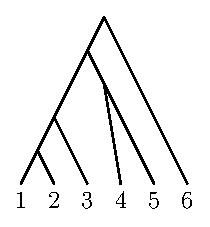
\includegraphics[width=0.4\textwidth]{ranked_tree}
\vspace{12pt}
\caption{A ranked tree with $6$ taxa.}
\label{fig:ranked_tree}
\end{figure}

We investigate the geometry and algorithmic complexity of the $\rnni$ space.
Specifically, in this paper we establish the exact radius and diameter of the space (Section~\ref{section:diameter}).
We also show that the subset of caterpillar trees is convex in $\rnni$ (Section~\ref{section:caterpillar_convex}), thus settling one of the open problems proposed in \autocite{Gavryushkin2018-ol}.
For establishing these geometric properties we use algorithms that will be introduced in Section~\ref{section:algorithms}.
We will in particular provide an approximate algorithm that computes exact distances for small trees.
The question of whether there exists a polynomial algorithm for computing the $\rnni$ distance remains an open problem.

In the rest of this chapter we formally introduce the terminology used in this paper.

A \emph{ranked phylogenetic tree} is a pair consisting of a rooted binary phylogenetic tree $T$ on the set $X = \{1, \ldots, n\}$ of \emph{taxa} for $n \in \mathbb N$, and a (total) rank function that maps all leaves of $T$ to $0$, all internal nodes of $T$ onto elements of the set $\{1, \ldots, n-1\}$, and respects the partial order on the nodes given by the tree.
The latter means that if $u$ and $v$ are two internal nodes of $T$ such that there exists a path from a taxon $x \in X$ to the root which first passes through $u$ and then through $v$ then $\rank(u) < \rank(v)$.
This definition also implies that the rank of every internal node is distinct and every $i$ with $1 \leq i \leq n-1$ equals the rank of some node.
Ranked trees $(T_1, \rank_1)$ and $(T_2, \rank_2)$ are different if trees $T_1$ and $T_2$ are different or $T_1 = T_2$ and $\rank_1 \neq \rank_2$.
Since all trees in this paper are ranked trees, we will abuse the notation and drop the rank function from the notation.
We will also simply say trees to mean ranked phylogenetic trees.
For a tree $T$, we will use $\rank_T$ to refer to its ranking.
A ranked tree $T$ without its leaf labels will be called \emph{tree topology}.

Our definition of a ranked tree implies a natural notion of edge length -- we call the difference in rank $|\rank_T(v) - \rank_T(u)|$ the length of an edge $(u, v)$.
We assume that edges of trees are undirected, so $(u, v) = (v, u)$.

Now we are ready to introduce the tree space which is the subject of study in this paper, the $\rnni$ graph.

The vertex set of the $\rnni$ graph is the set of all ranked trees on $n$ taxa.
We introduce two types of operation ($\rnni$ \emph{moves}) on trees (see Figure~\ref{fig:RNNI}) and say that two trees are adjacent in the $\rnni$ graph if one can be obtained from the other by an operation of either type.
The first type of operation is called a \emph{rank move} and defined by swapping the ranks of two internal nodes that are not adjacent in the tree.
Formally, if $u$ and $v$ are nodes of a tree $T$ such that $|\rank_T(u) - \rank_T(v)| = 1$ and $(u, v)$ is not an edge in $T$ then the tree $R$ obtained from $T$ by only changing $\rank_R(u) = \rank_T(v)$ and $\rank_R(v) = \rank_T(u)$ is said to be obtained by a rank move.
The second type of operation is called an $\nni$ \emph{move} and defined in the usual way, that is, two trees $T$ and $R$ are said to be connected by an $\nni$ move if there exist internal edges $e$ in $T$ and $f$ in $R$ both of length one such that the trees obtained by shrinking $e$ and $f$ to internal nodes coincide.

We use the notation $d(T, R)$ throughout the paper to denote the length of a shortest $\rnni$ path between tree $T$ and $R$.
An important geometric property analysed in this paper is whether trees from a certain class are connected but shortest paths that do not leave the class.
We say that a subset $S$ of trees is \emph{convex} if every pair of trees from $S$ is connected by a shortest path that completely stays within $S$.

\begin{figure}[H]
\centering
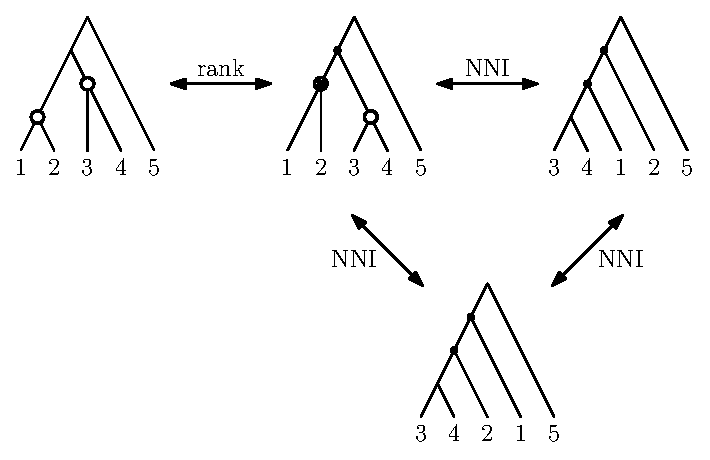
\includegraphics[width=0.8\textwidth]{RNNI}
\vspace{12pt}
\caption{Two types of operation that define edges of the $\rnni$ graph.
The rank move swaps the rank of the two highlighted nodes and the $\nni$ moves are performed on the dashed edges.}
\label{fig:RNNI}
\end{figure}

The rest of this paper is organised as follows.
In Section~\ref{section:algorithms} we introduce three algorithms for exploring the $\rnni$ graph.
We use these algorithms in Section~\ref{section:geometry} to establish several geometrical properties of this graph, such as its diameter and radius.
Furthermore, we will establish in Section~\ref{section:caterpillar_convex} that a certain subspace of $\rnni$ is convex and design a polynomial-time algorithm for computing $\rnni$-distances in that subspace.
This result suggests that the complexity of computing distances in $\rnni$ is different from that in the classical $\nni$ space.
We will discuss this further in Section~\ref{section:cluster_theorem}, where we disprove a conjecture of \textcite{Gavryushkin2018-ol} and suggest weaker versions as plausible alternatives.
In Section~\ref{section:partition_lattice} we establish a connection between the $\rnni$ graph and a classical algebraic structure, the partition lattice.
We will finish the paper with a discussion and open problems.


\section{Algorithms}
\label{section:algorithms}

In this section we introduce three algorithms, $\findpath$ (Section~\ref{section:alg_findpath}), $\csort$ (Section~\ref{section:alg_csort}), and $\mdtree$ (Section~\ref{section:alg_mdtree}).
$\findpath$ computes an $\rnni$ path between trees.
$\csort$ computes a shortest $\rnni$ path between caterpillar trees (also known as ladder trees, see later in this section for formal definitions).
$\mdtree$ attempts to maximise the dissimilarity to find a remote tree from an arbitrary $\rnni$ tree.
While these algorithms are interesting on their own (e.g.\ in simulation studies), they will also form an important ingredient to study the geometry of the $\rnni$ space later in this paper.
For example, $\mdtree$ will be an important tool for finding the radius of the $\rnni$ graph, as the algorithm computes a tree with maximum distance if the input tree is a caterpillar tree.
We will prove this fact in Section~\ref{section:diameter}.

The algorithm $\findpath$ can be used to approximate the $\rnni$ distance.
We will study the accuracy of this approximation by computing the exact $\rnni$ distance for small trees.
Specifically, we will use the algorithm for computing the complete $\rnni$ graph that is given in \autocite[Section 3.3]{Gavryushkin2018-ol}.
After pre-computing the graph, we use Seidel's algorithm \autocite{seidel_all-pairs-shortest-path_1995} for computing distances.
However, the large number of vertices in $\rnni$ is an obstacle when it comes to computing distances for larger trees.
Since there are $\frac{n!(n-1)!}{2^{n-1}}$ vertices in the $\rnni$ graph \autocite{Gavryushkin2018-ol}, we compute the $\rnni$ graph on up to seven taxa for our analyses.
This computational result will also be used later in the paper to support Conjecture~\ref{conjecture:cluster_theorem}, a modification of Conjecture~9 in \autocite{Gavryushkin2018-ol}, which we prove to be false in this paper.

Note that computing the $\rnni$ space on trees with seven taxa is a challenging goal to achieve.
For example, \textcite{Whidden2016-kl} were able to compute the much smaller $\spr$ space on up to seven taxa and used this to compute curvature values for all pairs of trees within that space.
%TODO: Make a zenodo dio for the repository before final publication
We have implemented all our algorithms in a combination of Python and C, and the source code is available at \autocite{Collienne2019}.


\subsection{$\findpath$}
\label{section:alg_findpath}

In this section we present $\findpath$, an efficient algorithm for computing paths, and therefore approximating distances, between trees in $\rnni$.

Before introducing the algorithm we need the following definitions.
Each node $v$ of a tree defines a \emph{cluster} $C$, which is the set of taxa descending from $v$.
We then say that $v$ \emph{induces} $C$.
All trees on $n$ leaves share trivial clusters, which are those induced by leaves and the root, so we exclude them from consideration and assume cluster means a non-trivial cluster.
A tree is unambiguously defined by the list of its clusters sorted according to the rank of the inducing nodes.
We will refer to this list of $n-2$ clusters for a given tree on $n$ taxa as a \emph{cluster representation} of the tree \autocite{Gavryushkin2018-ol, Gavryushkin2016-uu, Semple2003-nj}.

Let $T$ and $R$ be arbitrary trees and $[C_1, \ldots, C_{n-2}]$ be the cluster representation of $R$ (the ``destination'' tree).
Then $C_i$ is induced by the node of rank $i$ for $i = 1, \ldots, n-2$.
$\findpath$ computes a path by iteratively extending a sequence $p$ of trees starting from $T$.
The algorithm terminates when $p$ is an $\rnni$ path from $T$ to $R$.
At step $k = 1, \ldots, n-2$ of $\findpath$ we consider the cluster $C_k$ and extend path $p$ as follows.
We search for a node in the last tree $T'$ of $p$ from the previous step that induces the smallest cluster containing all elements of $C_k$.
This node is denoted by $\mrca_{T'}(C_k)$ (short for \emph{most recent common ancestor}).
We then extend $p$ by adding the tree obtained from $T'$ by performing an $\rnni$ move that decreases the rank of $\mrca_{T'}(C_k)$.
We continue extending $p$ in this way by repeatedly performing $\rnni$ moves until the rank of $\mrca_{T'}(C_k) = k$, thus completing step $k$.

\begin{algorithm}[H]
\caption{$\findpath$($T,R$)}
\begin{algorithmic}[1]
\STATE $T' := T$, $p := [T']$, $[C_1, \ldots, C_{n-2}] := R$
\FOR {$k = 1, \dots, n-2$}
    \WHILE {$\rank_{T'}(\mrca_{T'}(C_k))>k$}
        \IF {node $u$ with $\rank_{T'}(u) = rank_{T'}(\mrca_{T'}(C_k))-1$ is adjacent to $\mrca_{T'}(C_k)$}
            \STATE $T'$ is $T'$ with $\rank_{T'}(\mrca_{T'}(C_k))$ decreased by an $\nni$ move
        \ELSE
            \STATE $T''$ is $T'$ with ranks of $u$ and $\mrca_{T'}(C_k)$ swapped
        \ENDIF
        \label{alg:findpath:line:move_set_down}
        \STATE $T' = T''$
        \STATE $p = p+T'$
      \ENDWHILE
\ENDFOR
\RETURN $p$
\end{algorithmic}
\end{algorithm}

\begin{proposition}
$\findpath$ is a correct deterministic algorithm.
\end{proposition}

\proof
It suffices to show that the update operation (line~\ref{alg:findpath:line:move_set_down}) is well-defined, that is the $\rnni$ move that decreases the rank of $\mrca_{T'}(C_k)$ is unique.

Case $k = 1$.
In this case $C_k$ consists of two taxa $\{x, y\}$.
The node $v = \mrca_{T'}(x, y)$ has $\rank_{T'}(v) = r > 1$.
Consider the node $w$ preceding $v$ in $T'$, that is, $\rank_{T'}(w) = r - 1$.
If a rank move that swaps $v$ and $w$ is possible then this is the only move on $T'$ that can decrease the rank of $\mrca(x, y)$.
If the rank move is impossible then there is an edge in $T'$ connecting $v$ and $w$.
The only way to decrease the rank of $\mrca(x, y)$ then is to perform an $\nni$ move on that edge.
It is not hard to see that out of two possible $\nni$ moves only one decreases the rank of this $\mrca$.

Case $k > 1$.
\begin{enumerate}
\item $C_k = C_i \cup C_j$ for $i, j < k$.
Suppress $C_i$ and $C_j$ in both $T'$ and $R$ to new taxa $c_i$ and $c_j$ respectively and proceed as in Case $k = 1$.
\item $C_k = C_i \cup \{x\}$, where $x$ is a taxon not present in $C_1, \ldots, C_k$.
Suppress $C_i$ in both $T'$ and $R$ to a new taxon $c_i$ and proceed as in Case $k = 1$.
\item $C_k = \{x, y\}$ where both $x$ and $y$ are not in $C_1, \ldots, C_k$.
Proceed as in Case $k = 1$.
\end{enumerate}
\endproof

Clearly, the worst-case complexity of $\findpath$ is quadratic in the number of taxa.

Because the algorithm returns a path between pairs of trees in $\rnni$, the length of the path approximates the $\rnni$ distance from above.
A natural question then is how accurate this approximation is.
We have computationally shown that the algorithm $\findpath$ finds the correct distance for trees up to seven taxa \autocite{Collienne2019} and know of no larger counterexample.


\subsection{$\csort$}
\label{section:alg_csort}

In this section we introduce an algorithm to compute paths between \emph{caterpillar trees}, which are trees where each internal node is adjacent to at least one leaf.
As a result caterpillar trees have only one \emph{cherry}, which is a pair of taxa that share their parent.
A path between two caterpillar trees that only consists of caterpillar trees is called a \emph{caterpillar path}.
We can identify a caterpillar tree $T = [\{x_1, x_2\}, \{x_1, x_2, x_3\}, \ldots, \{x_1, \ldots, x_{n-1}\}]$ with the list of its taxa $[x_1, x_2, \ldots, x_n]$, assuming that $x_1 < x_2$ (recall that the set of taxa is $\{1, \ldots, n\}$).

The algorithm $\csort$ (Algorithm~\ref{alg:csort}) is a modification of the classical Bubble Sort algorithm \autocite{Knuth1997-pi}.
A path $p$ from $T$ to $R= [x_1, \ldots, x_n]$ is computed iteratively so that after $k$ steps the last $k$ taxa of $T$ and $R$ coincide.
Specifically, in step $k$ ($k = n, \ldots, 3$) the parent of taxon $x_{k}$ is moved up by $\nni$ moves to the position it has in $R$.
Notice that there might be more than just one such move per step, which means that $p$ can be extended by more than one tree in each step.

\begin{algorithm}[H]
\caption{$\csort$($T,R$)}
\label{alg:csort}
\begin{algorithmic}[1]
\STATE $[x_1, x_2, \ldots, x_n] := R$, $T' := T$, $p = [T']$
\FOR {$k=n, \ldots, 3$}
    \FOR {$i=1, \ldots, k$}
        \IF {taxon $T'[i]$ at position $i$ in $T'$ equals $x_k$}
            \STATE $T''$ is $T'$ with $T'[i]$ and $T'[i+1]$ swapped
            \STATE $T' = T''$
            \STATE $p = p + T'$
        \ENDIF
    \ENDFOR
\ENDFOR
\RETURN $p$
\end{algorithmic}
\end{algorithm}

The running time of $\csort$ is quadratic in $n$.

The path $p$ returned by $\csort$ is a shortest caterpillar path because every tree modification on $p$ reduces the number of inversions of taxa in $T$ and $R$, and no modification can reduce more than one insertion.
Indeed, no $\rnni$ move on caterpillar trees can reduce the number of taxa inversions by more than one, assuming that inversions with both taxa of a cherry are counted only once.
That is, if both pairs of taxa $(x, z)$ and $(y, z)$ appear in opposite orders in $T$ and $R$ and $x$ an $y$ form a cherry then they are counted as one inversion.
Notice that because of this the distance between caterpillar trees does not coincide with the Kendall tau distance \autocite{Kendall1948-tx}, counting the number of pairs of elements that appear in different order in two permutations, even though the idea is very similar.
Hence any caterpillar path, every move along which reduced the number of inversions, is a shortest caterpillar path.

It is not obvious that the path between $T$ and $R$ returned by $\csort$ has the least possible length among all $\rnni$ paths (not only caterpillar paths), that is, the length of $d(T, R)$.
This fact will be established in Theorem~\ref{thm:caterpillar_convex}.

Our Python implementation of this algorithm can be accessed at \autocite{Collienne2019}.


\subsection{$\mdtree$}
\label{section:alg_mdtree}

The idea behind this algorithm is to efficiently return a tree as far away from a given tree as possible.
As we will see in Section~\ref{section:diameter}, $\mdtree$ achieves this goal for caterpillar trees.

$\mdtree$ (Algorithm~\ref{alg:max_dist_tree}) works as follows.
Given an arbitrary tree $T$, order its taxa in a list $L = [l_1, \ldots, l_n]$ so that the ranks of their parents are non-decreasing with respect to this order.
Note that this list is not uniquely determined by the tree.
$\mdtree$ constructs an output tree $R$ as follows:
Initially, $R$ only consists of two taxa $l_1$ and $l_2$, the most recent common ancestor of which will eventually be of rank $n - 1$.
The remaining taxa are iteratively added to $R$ reversing the order of $L$.
At every iteration, the taxon is attached to a new internal node created on one of the existing branches in $R$ so that this new attachment node has rank one.
Note that $R$ is not uniquely determined due to the non-deterministic choice of the attachment edge.

\begin{algorithm}[H]
\caption{$\mdtree(T)$}
\label{alg:max_dist_tree}
\begin{algorithmic}[1]
\STATE Construct list $L=[l_1, \ldots, l_n]$ of all taxa ordered with respect to the ranks of their parents in $T$
\label{alg:mdtree_lineL}
\STATE Build tree $R$ with two taxa $l_1, l_2$ that are children of the root
\FOR {$i = 3, \ldots, n$}
\STATE Extend $R$ by attaching $l_i$ to a newly created node of rank $1$ on an arbitrarily chosen edge
\label{alg:mdtree_lineAddTaxon}
\ENDFOR
\RETURN $R$
\end{algorithmic}
\end{algorithm}

Note that the list computed in Line~\ref{alg:mdtree_lineL} of $\mdtree$, as well as the attachment edge of the new taxon in Line~\ref{alg:mdtree_lineAddTaxon} are not uniquely determined.
Therefore, this algorithm is non-deterministic, which is an important observation that we will use for finding the radius of $\rnni$ in Section~\ref{section:diameter}.


\section{Geometry of $\rnni$}
\label{section:geometry}

The study of shortest paths in the $\rnni$ graph in this section is motivated by our aim to understand the geometry of $\rnni$ as a metric space.
We will employ the algorithms developed in the previous section to aid our analysis of shortest paths.
Those algorithms will, for example, enable us to prove that the set of caterpillar trees is convex in $\rnni$ (Theorem~\ref{thm:caterpillar_convex} in Section~\ref{section:caterpillar_convex}).
In Section~\ref{section:diameter} we will investigate the diameter and radius of the $\rnni$ space.
Interestingly, the \emph{diameter} of $\rnni$, that is the maximum distance $\Delta(\rnni) = \max \{d(T, R) \mid T, R \in \rnni\}$ between any two trees in the graph, equals its \emph{radius} defined as $\min\limits_T \max\limits_R d(T,R)$.
Next, we will consider the so-called Split Property \autocite{Gavryushkin2018-ol}, that is, every shared split of taxa is maintained along every shortest path.
Recall that a \emph{split} is a bipartition of the set of taxa obtained by deleting an edge of the tree $T$.
Splits are denoted by $A|B$.
We will give a counterexample to show that $\rnni$ does not have the Split Property and consider a variant, the Weak Split Property, which says that every shared split of taxa is maintained along a shortest path.
We will also consider the so-called Cluster Property as another weak version of the Split Property (see Conjecture~\ref{conjecture:cluster_theorem}).
In the final part of this geometry section we will discuss the relation between the $\rnni$ graph and the so-called partition lattice, a well known algebraic structure.

We start with the following auxiliary results.

\begin{lemma}
$\Delta(\rnni) \leq \frac{(n-1)(n-2)}{2}$ for $n \geq 3$.
\label{lemma:diameter_bound}
\end{lemma}

\begin{proof}
Since the diameter is bounded from above by the maximum length of a path computed by $\findpath$, it is enough to find this maximum.
Let us assume that $T$ and $R = [C_1, \ldots, C_{n-2}]$ are trees for which $\findpath$ computes a path of maximum length.
It follows that in each step of $\findpath$ the most recent common ancestor of the cluster $C_k$ considered in that step is the root.
Thus, there are $n-1-k$ $\rnni$ operations necessary to move $C_k$ to its correct position.
Hence, the maximum length of a path computed by $\findpath$ is bounded by $\sum\limits_{i = 1}^{n-2} (n-1-i) = \frac{(n-2)(n-1)}{2}$.
\end{proof}

The following lemma relates distances between trees on $n$ and $n+1$ taxa and is an important tool for inductive arguments.
We use the notion $\parent_T(x)$ to refer to the node adjacent to taxon $x$ in tree $T$.
Let $T{\big|}_n$ denote the restriction of tree $T$ to the set of taxa $\{1, \ldots, n\}$.
In other words, if $T$ is a tree on taxa $\{1, \ldots, n+1\}$ the tree $T{\big|}_n$ is obtained by deleting taxon $n+1$ and suppressing the thereby created node of degree two, updating node rankings accordingly.

\begin{lemma}
Let $T$ and $R$ be two trees on taxa $\{1, \ldots, {n+1}\}$.
Then ${d(T{\big|}_n, R{\big|}_n) \leq d(T,R) - \delta}$, where $\delta = |\rank_T(\parent_T(n+1)) - \rank_R(\parent_R(n+1))|$.
\label{lemma:distance_delete_taxon}
\end{lemma}

\begin{proof}
First observe that the rank of the internal node $\parent_T(n+1)$ can only be changed by performing a rank move that involves $\parent_T(n+1)$ or an $\nni$ move on an edge adjacent to $\parent_T(n+1)$.
Second observe that any $\rnni$ move can change the rank of $\parent_T(n+1)$ by at most one.
Hence an $\rnni$ move on $T$ can decrease the rank of $\parent_T(n+1)$ by at most one.

Let $p$ be a shortest path from $T$ to $R$ and $p{\big|}_n$ the path resulting from deleting taxon $n+1$ from all trees on $p$ and removing all identical trees.
Then $p{\big|}_n$ is a path from $T{\big|}_n$ to $R{\big|}_n$.
Recall that $\delta$ is the difference in ranks between the parents of taxon $n+1$ in $T$ and $R$.
Combining this with the observations above, we conclude that $|p{\big|}_n| \leq |p| - \delta$.
Since $d(T{\big|}_n,R{\big|}_n) \leq |p{\big|}_n|$ and $|p| = d(T,R)$, the desired inequality follows.
\end{proof}


\subsection{The set of caterpillar trees}
\label{section:caterpillar_convex}

In this section we restrict our attention to the set of caterpillar trees.
These trees are of particular interest because they are used to prove that computing $\nni$ distances is an NP-hard problem.
As we will see below, shortest paths between caterpillar trees in the $\rnni$ space differ from those in the classical $\nni$ space.
We will show later in this section that $\rnni$ distances between caterpillar trees can be computed in polynomial time.
Throughout this section we use the list representation of caterpillar trees described in Section~\ref{section:alg_csort}.

\textcite{Gavryushkin2018-ol} showed that computing a shortest path between two caterpillar trees in the $\nni$ graph sometimes requires first building a clade and then moving the clade around the tree (see Figure~\ref{fig:NNI_vs_RNNI}).
In the $\rnni$ graph however, the necessity of additional rank moves invalidates this strategy.
This is due to the fact that $\nni$ moves in $\rnni$ are only allowed on edges of length one.

\begin{figure}[H]
\centering
\includegraphics[width=\textwidth]{NNI_vs_RNNI}
\vspace{12pt}
\caption{Paths between caterpillar trees $T$ and $R$: Solid arrows indicate paths in $\rnni$, the dashed arrow is a move only possible in $\nni$.
The bottom path is a shortest $\rnni$ path.}
\label{fig:NNI_vs_RNNI}
\end{figure}

These observations motivate the following general result.
We will show that every pair of caterpillar trees $T, R$ in $\rnni$ are connected by a caterpillar path of length $d(T,R)$, that is, the set of caterpillar trees is convex in $\rnni$ (Theorem~\ref{thm:caterpillar_convex}).
Note that this is not true in the $\nni$ space (Figure~\ref{fig:NNI_vs_RNNI}).

For proving the convexity of the set of caterpillar trees we need the following lemma.
Recall that $\frac{(n-1)(n-2)}{2}$ is an upper bound of the diameter of $\rnni$ by Lemma~\ref{lemma:diameter_bound}.

\begin{lemma}
Let $T$ and $R$ be two caterpillar trees.
Then $d(T,R) = \frac{(n-1)(n-2)}{2}$ if and only if $d_c(T,R) = \frac{(n-1)(n-2)}{2}$, where $d_c$ is the length of a shortest caterpillar path.
\label{lemma:caterpillar_dist=diameter}
\end{lemma}

\begin{proof}
First note that $d(T,R) = \frac{(n-1)(n-2)}{2}$ implies $d_c(T,R) \geq \frac{(n-1)(n-2)}{2}$.
In each step $i=0, \ldots, n-3$ of $\csort$ at most $n-2-i$ pairs of taxa swap positions, as in the worst case the taxon considered in step $k$ is moved from the cherry of the tree up to the position $n-k$.
It follows that the maximum length of a path computed by $\csort$ is
\begin{equation}
\sum\limits_{i=0}^{n-3} (n-2-i) = \frac{(n-1)(n-2)}{2},
\label{csort_max}
\end{equation}

so $d_c(T,R) = \frac{(n-1)(n-2)}{2}$

To prove the converse, assume that $d_c(T,R) = \frac{(n-1)(n-2)}{2}$.
We prove that $d(T,R) = \frac{(n-1)(n-2)}{2}$ by induction on the number of taxa $n$.
The induction basis for $n=3$ taxa is trivial as the $\rnni$ graph is a triangle on three caterpillar trees in this case.

For the induction step we assume without loss of generality that $T$ is the caterpillar tree $[1, \ldots, n+1]$ and $R$ is a caterpillar tree such that $d_c(T, R) = \frac{n(n-1)}{2}$.
Consider the path $p = \csort(T, R)$ of this length.
Note that in this case taxon $n+1$ has to be in the cherry of $R$, as otherwise $\csort$ would find a path between $T$ and $R$ of length strictly less than $\frac{n(n-1)}{2}$, which can be shown by counting the number of moves as in (\ref{csort_max}) above.

Let us now consider the path $p\big|_n$ from $T\big|_n$ to $R\big|_n$, which is obtained by restricting every tree on $p$ to taxa $1, \ldots, n$ and removing identical trees.
Observe that this path is shorter than $p$ by the number of moves that involve taxon $n+1$.
Since this taxon is adjacent to the root in $T$ and part of the cherry in $R$, $\csort$ requires $n-1$ such moves.
Hence, $d_c(T{\big|}_n, R{\big|}_n) = \frac{n(n-1)}{2} - (n-1)$ = $\frac{(n-1)(n-2)}{2} = d(T{\big|}_n,R{\big|}_n)$, by the induction hypothesis.
Lemma~\ref{lemma:distance_delete_taxon} implies that $d(T{\big|}_n, R{\big|}_n) \leq d(T,R) - |\rank_T(\parent_T(n+1)) - \rank_R(\parent_R(n+1))| = d(T,R) - (n-1)$.
So $\frac{(n-1)(n-2)}{2} \leq d(T,R) - (n-1)$, which implies that $d(T, R) \geq \frac{n(n-1)}{2}$.
Thus $d(T, R) = \frac{n(n-1)}{2}$.
\end{proof}

\begin{theorem}
The set of caterpillar trees is convex in $\rnni$.
\label{thm:caterpillar_convex}
\end{theorem}

\proof
Note that it suffices to prove that $d_c(T, R) = d(T, R)$ for an arbitrary pair of caterpillar trees $T$ and $R$.
Lemma~\ref{lemma:caterpillar_dist=diameter} implies that if $T$ and $R$ are at the maximal possible distance, it is $d_c(T, R) = \frac{(n-1)(n-2)}{2}$.
Denote the latter number by $D$.

Assume now that $d_c(T, R) = D - 1$.
If we apply $\csort(T, R)$ in this case, there must be a step in the algorithm where the taxon that is moved up is not part of the cherry (of $T'$) at the beginning of this step.
Let $x$ be the first taxon that has this property and is considered at step $k$.
Then there must be a taxon $y$ that is immediately preceding $x$ in the tree at the beginning of step $k$.
Since $k$ is the first such step, $y$ must be preceding $x$ in tree $T$ as well.
Consider a tree $\hat T$ that is obtained from $T$ by exchanging $x$ and $y$.
Note that the caterpillar path from $\hat T$ to $R$ computed by $\csort$ passes $T$ and coincides with the path $\csort(T, R)$ from there on.
Clearly, $d_c(\hat T, R) = D$.

Assuming $d_c(T, R) < D$, we can iterate the construction above to find a tree $\hat T$ such that $d_c(\hat T, R) = D$ and the caterpillar path from $\hat T$ to $R$ computed by $\csort$ passes $T$ and coincides with the path $\csort(T, R)$ from there on.
Lemma~\ref{lemma:caterpillar_dist=diameter} implies that $d(\hat T, R) = D$.

Assume that $d(T, R) < d_c(T, R)$ and let $p$ be a path from $T$ to $R$ of length $d(T, R)$.
Consider a path $q$ obtained by concatenating paths $\csort(\hat T, T)$ and $p$.
Note that $q$ is a path from $\hat T$ to $R$ which is shorter than $\csort(\hat T, R)$.
Indeed, the two paths coincide between $\hat T$ and $T$, and $q$ is shorter between $T$ and $R$.
Since $d_c(\hat T, R) = D$, the existence of $q$ is a contradiction of Lemma~\ref{lemma:caterpillar_dist=diameter}.
\endproof


\subsection{Diameter and radius}
\label{section:diameter}

\textcite[Theorem~7]{Gavryushkin2018-ol} gave an upper bound for the diameter of $\rnni$ space, denoted by $\Delta(\rnni)$.
They showed that $\Delta(\rnni) \leq n^2 - 3n - 5/8$.
In this section we improve that result and calculate the exact diameter and radius of the $\rnni$ space.

\begin{theorem}
$\Delta(\rnni) = \frac{(n-1)(n-2)}{2}$.
\label{thm:diameter}
\end{theorem}

\proof
Since $d_c([1\ldots,n], [n-1,n,n-2,n-3, \ldots, 1]) = \frac{(n-1)(n-2)}{2}$, the claim follows directly from Theorem~\ref{thm:caterpillar_convex} and Lemma~\ref{lemma:diameter_bound}.
\endproof

We show in the rest of this section that the radius of $\rnni$ space coincides with its diameter.
The main tool to establish this result is the algorithm $\mdtree$ from Section~\ref{section:alg_mdtree}.
Recall that $\mdtree$ is a non-deterministic algorithm, which implies that the output tree is not uniquely defined by the input to the algorithm.

\begin{lemma}
Let $T$ be a caterpillar tree.
Then $d(T, R) = \Delta(\rnni)$ for every tree $R$ such that $R = \mdtree(T)$.
\label{lemma:max_dist_caterpillar}
\end{lemma}

\begin{proof}
We prove the lemma by induction on the number of taxa $n$.
The induction basis for $n = 3$ is trivial.

Assume now that $T = [1, \ldots, n+1]$.
In this case, the parent of taxon $n+1$ has rank $n$ in $T$ and rank $1$ in $R$.
Lemma~\ref{lemma:distance_delete_taxon} then implies that
\begin{equation}
d(T\big|_n,R\big|_n) \leq d(T,R) - (n-1).
\label{eqn:max_dist_cat_proof}
\end{equation}
Note that $R\big|_n = \mdtree (T\big|_n)$ for an appropriate choice of attachment points in the execution of $\mdtree$.
By the induction hypothesis and Theorem~\ref{thm:diameter}, $d(T\big|_n,R\big|_n) = \frac{(n-1)(n-2)}{2}$.
So inequality~(\ref{eqn:max_dist_cat_proof}) becomes $d(T,R) \geq \frac{(n-1)(n-2)}{2} + n - 1 = \frac{n(n-1)}{2}$, which gives the desired equality with Theorem~\ref{thm:diameter}.
\end{proof}

The non-determinism of $\mdtree$ can be exploited to investigate which trees are at the maximal possible distance from a given caterpillar tree.
In fact, those trees can have an arbitrary (non-ranked) topology.
This is because in each step of the algorithm the next taxon can be added on any edge incident to a leaf in the running tree.
Therefore, $\mdtree$ can be used to find a tree of pre-defined topology that is at the maximal possible distance from the input tree, in particular if the input is a caterpillar tree.
Because the distance between trees is invariant under permutations of taxa labels, we conclude that for every tree $R$ on $n$ taxa there exists a caterpillar tree $T$ such that $d(T,R) = \Delta(\rnni) = \frac{(n-1)(n-2)}{2}$.
This proves the following Theorem~\ref{thm:radius}.

\begin{theorem}
The radius and diameter of the $\rnni$ space coincide and are equal to $\frac{(n-1)(n-2)}{2}$.
\label{thm:radius}
\end{theorem}


\subsection{Cluster Property}
\label{section:cluster_theorem}

In this section we discuss the so-called Split Property, which states that every split shared between two trees is maintained along shortest paths between the trees.
For example, the $\spr$ space has the Split Property while $\nni$ does not \autocite{Li1996-zw}.
Specifically, in $\nni$ there exist two trees $T$ and $R$, which share a split $A | B$, such that every tree on every shortest path between $T$ and $R$ does not have $A | B$.

To construct this example, \textcite{Li1996-zw} used the idea illustrated in Figure~\ref{fig:NNI_NP_proof} and showed that for an appropriate permutation of the taxa in the two caterpillar subtrees of both $T$ and $R$, it is strictly shorter to merge the two caterpillar subtrees first, then sort them simultaneously, and then split back to two caterpillar subtrees, rather the two caterpillar subtrees independently.

The reason this example cannot be transferred to $\rnni$ is that additional rank moves are necessary to merge and then split the two caterpillar subtrees.
Similarly to the example in Figure~\ref{fig:NNI_vs_RNNI}, adding rank moves to the shortest $\nni$ path from $T$ to $R$ results in a path that is not a shortest $\rnni$ path.
Sorting the two caterpillar subtrees of $T$ and $R$ independently results in a shorter path in $\rnni$.

\begin{figure}[H]
\centering
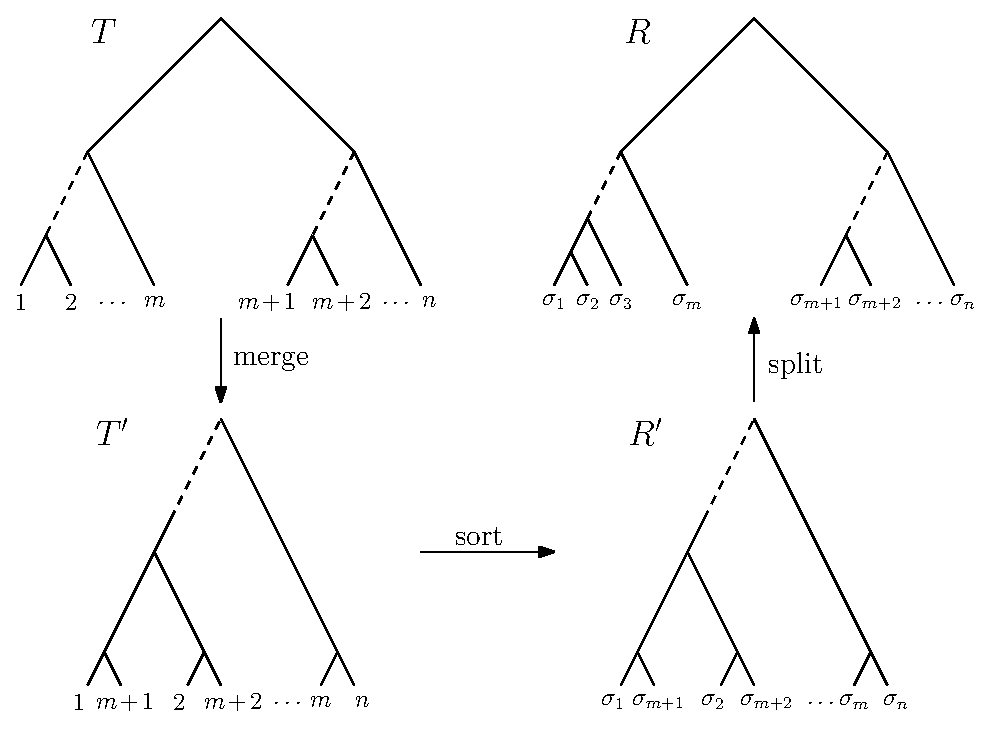
\includegraphics[width=.8\textwidth]{NNI_NP_proof}
\vspace{12pt}
\caption{Example of a shortest path between two trees $T$ and $R$ in $\nni$.
In \autocite{Li1996-zw} it is proven that there is a labelling that ensures that there is no shortest path in $\nni$ where the clusters $\{1, \ldots, m\}$ and $\{m+1, \ldots, n\}$ with $m = \frac{n}{2}$ shared between $T$ and $R$ are preserved.
Instead, the depicted path where $\frac{n}{2}$ cherries are built and then sorted before being resolved is a shortest path}
\label{fig:NNI_NP_proof}
\end{figure}

This argument motivated \textcite[Conjecture~9]{Gavryushkin2018-ol} to conjecture that every split shared between trees in $\rnni$ is maintained along every shortest path.

The example in Figure~\ref{fig:splitthm_counterexample} shows that, in this form, the Split Property is not present.

\begin{figure}[H]
\centering
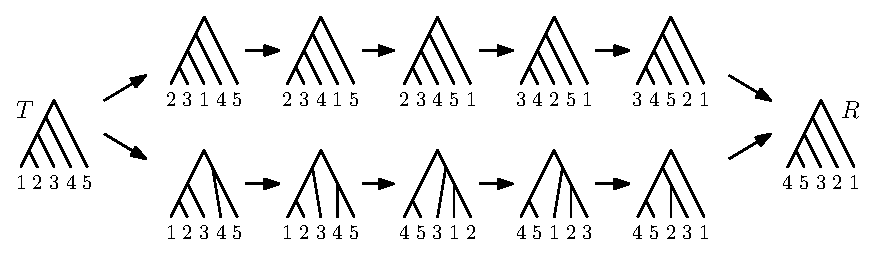
\includegraphics[width=\textwidth]{splitthm_counterexample}
\vspace{12pt}
\caption{The split $123|45$ is present in $T$ and $R$, but the path at the top is a shortest path (computed by $\csort$) where none of the trees contains this split.
On the path at the bottom, which is a shortest path as well, this split is maintained.}
\label{fig:splitthm_counterexample}
\end{figure}

Hence not every shortest path between trees in $\rnni$ has to maintain every shared split of taxa.
However, there exists yet another shortest path connecting the two trees, along which every shared split is maintained.
This motivates the study of the following Weak Split Property in $\rnni$.

\begin{definition}[Weak Split Property]
If a split of taxa $A | B$ is shared by two trees $T$ and $R$ then there exists a shortest path $p$ between $T$ and $R$ such that all trees on $p$ share the split $A | B$.
\end{definition}

\begin{conjecture}
\label{conjecture:weak_split_theorem}
$\rnni$ has the Weak Split Property.
\end{conjecture}

Another interesting property of our counterexample in Figure~\ref{fig:splitthm_counterexample} is that the set of taxa $\{1, 2, 3\}$, which is a part of the split in both $T$ and $R$, does not form a cluster in $R$, that is, there is no single node in the tree all descended taxa of which are exactly $1$, $2$, and $3$.
Importantly, rooted phylogenetic trees can be uniquely represented by sets of clusters \autocite{Steel2016-ye}, but not by sets of splits as splits cannot define the position of the root.
For example, trees $T$ and $R$ in Figure~\ref{fig:splitthm_counterexample} induce the same set of splits, but share no cluster.

Furthermore, all our methods in this paper for computing shortest paths in special subspaces of $\rnni$ demonstrate that shared clusters are maintained along shortest paths.

These considerations motivate us to conjecture the following Cluster Property.

\begin{definition}[Cluster Property]
Let $T$ and $R$ be trees that share a cluster $C$.
Then $C$ is present as a cluster in every tree on every shortest path between $T$ and $R$.
\end{definition}

\begin{conjecture}
\label{conjecture:cluster_theorem}
$\rnni$ has the Cluster Property.
\end{conjecture}

We have found no counterexamples to this conjecture and have checked that it holds in $\rnni$ spaces with up to seven taxa ($n = 2, \ldots, 7$).
Specifically, we computed subgraphs of $\rnni$ containing only trees with shared clusters and compared distances in this subgraph with distances in the whole $\rnni$ graph.
We computed these graphs according to the algorithm from \autocite{Gavryushkin2018-ol} as discussed in Section~\ref{section:algorithms}.
The source code of all these implementations can be openly accessed at \autocite{Collienne2019}.


\subsection{Partition lattice}
\label{section:partition_lattice}

In this section we establish a connection between the $\rnni$ graph and a well known algebraic structure, the partition lattice.
The relation between these two provides a new direction for further research and leads to a different view on problems of either structure.

The \emph{partition lattice} on $\{1, \ldots, n\}$ is the lattice given by the partially ordered set $(\Pi_n,\leq)$, where $\Pi_n$ is the power set of $\{1, \ldots, n\}$ and $x \leq y$ if partition $x$ refines $y$.
For simplification we will denote the partition lattice by $\Pi_n$, $\Pi_4$ is illustrated in Figure~\ref{fig:partition_lattice4}.
We assume that the partition lattice is ranked such that the partition into singletons has rank zero and the set $\{1, \ldots, n\}$ has rank $n-1$.
This algebraic structure is related to the $\rnni$ graph in the following way.

\begin{theorem}
The $\rnni$ graph on $n$ taxa is isomorphic to the graph of maximal chains of the partition lattice $\Pi_n$ where two maximal chains are connected by an edge if and only if they differ by exactly one partition.
The corresponding metric spaces are isometric.
\end{theorem}

\begin{proof}
There is a one to one relation between ranked trees and maximum chains in a partition lattice.
We can define a bijective mapping from the set of ranked trees to the set of maximum chains in $\Pi_n$ as follows.
A tree $T$ maps onto a maximum chain $\mathcal{C}_T$ if the set in the partition of rank $i$ in $\mathcal{C}_T$ that is the union of two sets of the partition of rank $i-1$ in $\mathcal{C}_T$ is the cluster induced by the internal node of rank $i$ in $T$.

An $\rnni$ move on a tree $T$ corresponds to changing exactly one partition on $\mathcal{C}_T$ as only one cluster changes by an $\rnni$ move on $T$.
From this we can follow that the $\rnni$ graph and the metric space on maximum chains of the partition lattice with this operation are isometric.
\end{proof}

\begin{figure}[H]
\centering
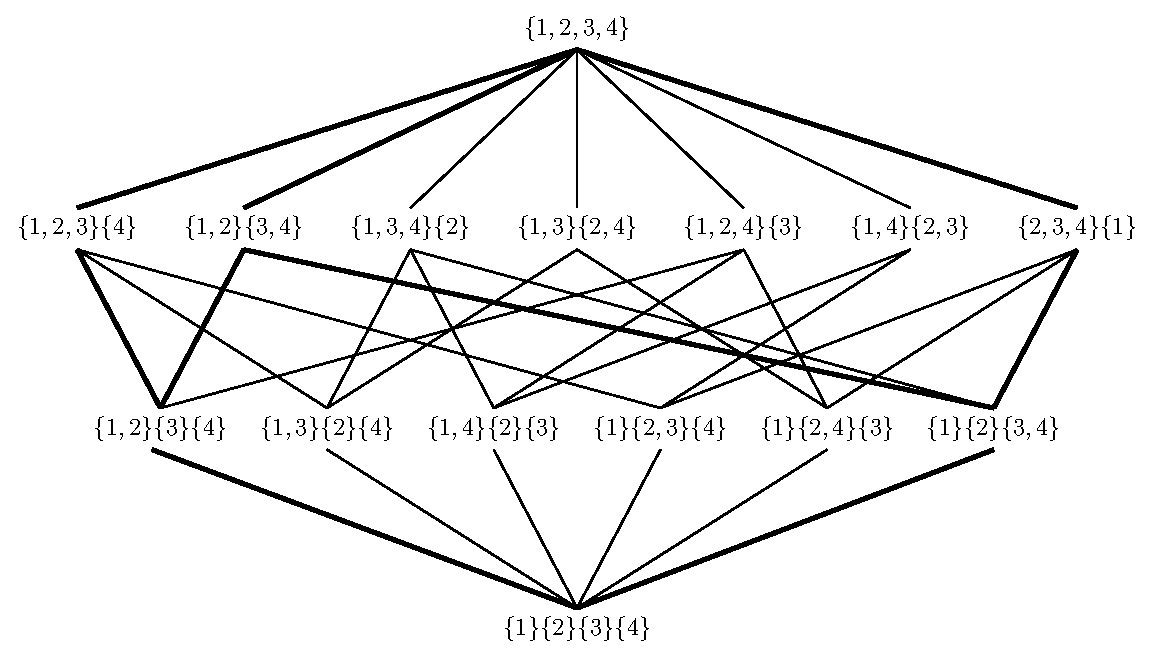
\includegraphics[width=\textwidth]{partition_lattice4}
\vspace{12pt}
\caption{The partition lattice $\Pi_4$ on $\{1,2,3,4\}$.
The highlighted edges correspond to an $\rnni$ path from the tree represented by the leftmost chain to the rightmost one.}
\label{fig:partition_lattice4}
\end{figure}


\section{Discussion}

The problem of computing distances in all common phylogenetic graphs, including $\nni$ \autocite{Dasgupta2000-xa}, $\spr$ \autocite{Bordewich2005-nx}, and $\tbr$ \autocite{Allen2001-ky}, is $\np$-hard.
Although $\np$-hardness does not necessarily imply practical impossibility, this so far has been the case for these phylogenetic algorithms with extremely few major advances \autocite{Whidden2010-bw}.
$\nni$ is especially known for its algorithmic hardness \autocite{Whidden2018-fw}.

Our results suggest a surprising advance in this field of $\np$-problems -- adding ranking information to trees simplifies some of the algorithms and makes some unintuitive counterexamples impossible.
We hence continued the investigation of the $\rnni$ graph on ranked phylogenetic trees in this paper.
We have taken the route of comparing the classic $\nni$ with the $\rnni$ graph, so have mostly been concentrating on questions that are settled in $\nni$.
Specifically, we have considered a number of geometric properties, including the diameter, radius, convexity of caterpillar trees, and the Split Property.
We have also justified that the technique of \textcite{Dasgupta2000-xa} to prove that distances in $\nni$ are $\np$-hard to compute cannot be directly applied in $\rnni$.
This led us to the Cluster Property, a statement that does not hold in $\nni$.
All our algorithms and methods developed in this paper witness in favour of $\rnni$ having the Cluster Property.
For example, we have checked the statement computationally for up to seven taxa \autocite{Collienne2019}.
Although the Split Property is present in $\spr$, it is still $\np$-hard to compute distances in that graph.
Hence the Cluster Property alone cannot be used as an argument in favour of the distance problem having an efficient solution in $\rnni$.
But the greedy nature of all our algorithms for computing shortest paths in $\rnni$ developed in this paper does provide such an argument.

The algorithms we developed and implemented in this paper have served as a main ingredient for our study of the geometry of $\rnni$ space.
These algorithms are of interest on their own as well.
For example, our $\findpath$ algorithm gives a good approximation of the $\rnni$ distance, performing exactly on small trees.
We are not aware of the minimal number of taxa where this algorithm fails to return the correct distance.
The $\mdtree$ algorithm produces trees as far away from a given tree as possible, a task of importance in simulation and model comparison studies.
The $\csort$ algorithm efficiently computes the $\rnni$ distance and shortest paths between caterpillar trees exactly.
To the best of our knowledge no such algorithm exists for $\nni$.
This implies that the algorithmic complexity of computing distances in $\nni$ is higher than in $\rnni$.

The question of whether computing $\rnni$ distances is $\np$-hard is still open.


\section*{Acknowledgements}
We thank Charles Semple for useful discussions about the Cluster Property, and Mike Steel for his useful comments that improved this paper.

We acknowledge support from the Royal Society of New Zealand through the Rutherford Discovery Fellowship (RDF-UOO1702) awarded to AG.
This work was partially supported by the Ministry of Business, Innovation, and Employment of New Zealand through the Endeavour Smart Ideas (CONT-61378-ENDSI-UOO) and Data Science Programmes grants.

MF thanks the joint research project \textit{DIG-IT!} supported by the European Social Fund (ESF), reference: ESF/14-BM-A55-0017/19, and the Ministry of Education, Science, and Culture of Mecklenburg-Vorpommern, Germany, for funding parts of this work.

Part of this work was done while AG, LC, and MF were visiting Max Plank Institute for Evolutionary Biology, we appreciate their support.


\printbibliography
\end{document}
